% Created 2024-09-12 ju. 21:54
% Intended LaTeX compiler: pdflatex
\documentclass[aspectratio=169, usenames,svgnames,dvipsnames]{beamer}
\usepackage[utf8]{inputenc}
\usepackage[T1]{fontenc}
\usepackage{graphicx}
\usepackage{longtable}
\usepackage{wrapfig}
\usepackage{rotating}
\usepackage[normalem]{ulem}
\usepackage{amsmath}
\usepackage{amssymb}
\usepackage{capt-of}
\usepackage{hyperref}
\usepackage{color}
\usepackage{listings}
\usepackage[spanish]{babel}
\setbeamercolor{alerted text}{fg=Blue}
\setbeamerfont{alerted text}{series=\bfseries}
\setbeamercolor{block title}{bg=structure.fg!20!bg!50!bg}
\setbeamercolor{block body}{use=block title,bg=block title.bg}
\AtBeginSubsection[]{\begin{frame}[plain]\tableofcontents[currentsubsection,sectionstyle=show/shaded,subsectionstyle=show/shaded/hide]\end{frame}}
\AtBeginSection[]{\begin{frame}[plain]\tableofcontents[currentsection,hideallsubsections]\end{frame}}
\lstset{keywordstyle=\color{blue}, commentstyle=\color{gray!90}, basicstyle=\ttfamily\small, columns=fullflexible, breaklines=true,linewidth=\textwidth, backgroundcolor=\color{gray!23}, basewidth={0.5em,0.4em}, literate={á}{{\'a}}1 {ñ}{{\~n}}1 {é}{{\'e}}1 {ó}{{\'o}}1 {º}{{\textordmasculine}}1, showstringspaces=false}
\usepackage{mathpazo}
\hypersetup{colorlinks=true, linkcolor=Blue, urlcolor=Blue}
\usepackage{fancyvrb}
\DefineVerbatimEnvironment{verbatim}{Verbatim}{fontsize=\tiny, formatcom = {\color{black!70}}}
\usepackage{pgfplots}
\usetheme{Boadilla}
\usecolortheme{rose}
\usefonttheme{serif}
\author{Francisco Delgado López}
\date{}
\title{Desarrollo de una herramienta software para la simulación de sistemas fotovoltaicos con R}
\subtitle{Trabajo de Fin de Grado}
\institute[UPM]{Universidad Politécnica de Madrid}
\beamertemplatenavigationsymbolsempty
\setbeamertemplate{footline}[frame number]
\setbeamertemplate{itemize items}[triangle]
\setbeamertemplate{enumerate items}[circle]
\setbeamertemplate{section in toc}[circle]
\setbeamertemplate{subsection in toc}[circle]
\hypersetup{
 pdfauthor={Francisco Delgado López},
 pdftitle={Desarrollo de una herramienta software para la simulación de sistemas fotovoltaicos con R},
 pdfkeywords={},
 pdfsubject={},
 pdfcreator={Emacs 29.2 (Org mode 9.6.15)}, 
 pdflang={Spanish}}
\begin{document}

\maketitle

\section{Introducción}
\label{sec:orgdbbb0d1}
\begin{frame}[label={sec:org478ff36},fragile]{Objetivo principal}
 \begin{block}{Desarrollo de un paquete en \texttt{R}}
\begin{lstlisting}[numbers=left,language=r,label= ,caption= ,captionpos=b]
library(solaR2)
\end{lstlisting}
\end{block}
\end{frame}

\begin{frame}[label={sec:org714719a},fragile]{Objetivos secundarios}
 \begin{block}{GNU Emacs}
\end{block}
\begin{block}{Paquetes de \texttt{R}}
\begin{itemize}
\item \texttt{solaR}
\item \texttt{zoo}
\item \texttt{data.table}
\item \texttt{microbenchmark}
\item \texttt{profvis}
\item \texttt{lattice}
\end{itemize}
\end{block}
\begin{block}{\LaTeX{}}
\end{block}
\begin{block}{Energía Solar Fotovoltaica}
\end{block}
\end{frame}

\section{Estado del arte}
\label{sec:org2b6d742}
\subsection{Sitación actual de la generación fotovoltaica}
\label{sec:org6392b84}

\subsection{Soluciones actuales}
\label{sec:org5163ded}
\begin{frame}[label={sec:orgabdf933}]{Soluciones actuales}
\begin{block}{\alert{PVsyst}}
\end{block}
\begin{block}{\alert{SISIFO}}
\end{block}
\begin{block}{\alert{PVGIS}}
\end{block}
\begin{block}{\alert{System Advisor Model}}
\end{block}
\end{frame}
\begin{frame}[label={sec:orga4f6543},fragile]{\texttt{solaR}}
 \begin{block}{Funcionamiento}
\begin{itemize}
\item Geometría solar
\item Datos meteorológicos
\item Radiación en el plano horizontal
\item Radiación en el plano del generador
\item Simulación de SFCR
\item Simulación de SFB
\item Optimización de distancias
\item Métodos de visualización
\end{itemize}
\end{block}
\end{frame}
\begin{frame}[label={sec:org4dfc101},fragile]{\texttt{solaR}}
 \begin{block}{Carencias}
\begin{itemize}
\item Modularidad
\item Eficiencia y rendimiento
\item Escalibilidad
\item Manipulación de datos
\end{itemize}
\end{block}
\end{frame}

\section{Marco teórico}
\label{sec:org284090f}
\begin{frame}[label={sec:org159cbd6}]{Procedimiento de cálculo}
\begin{center}
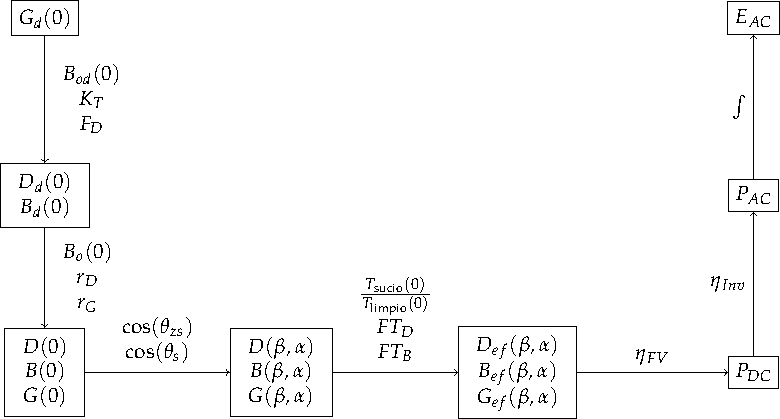
\includegraphics[scale=1]{../figuras/ProcedimientoCalculoRadiacionInclinada.pdf}
\end{center}
\end{frame}
\section{Desarrollo del código}
\label{sec:org0b2af3a}
\begin{frame}[label={sec:org1b1e7f0}]{Algorítmo de cálculo}
\begin{center}
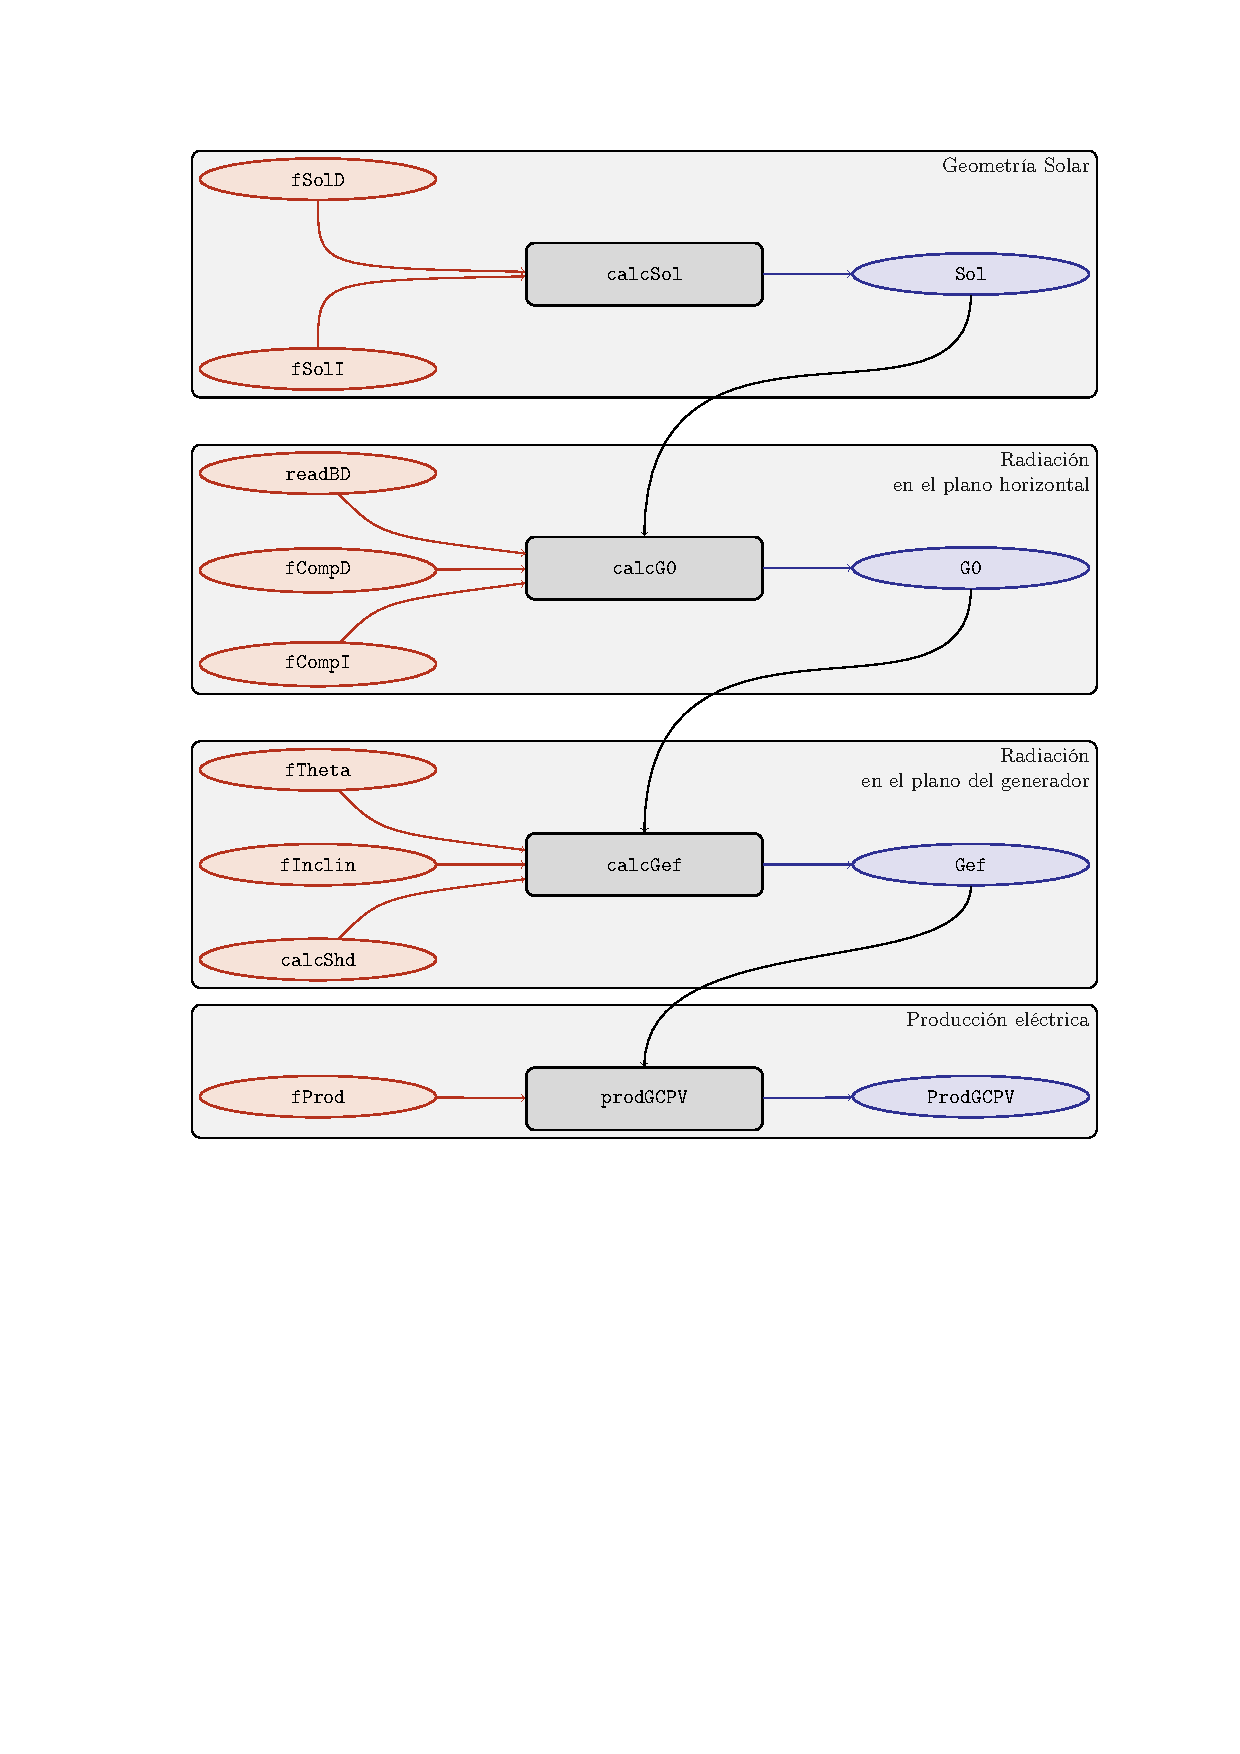
\includegraphics[height=0.9\textheight]{../figuras/procedure.pdf}
\end{center}
\end{frame}
\begin{frame}[label={sec:org3a273c7},fragile]{\texttt{calcSol}}
 \begin{center}
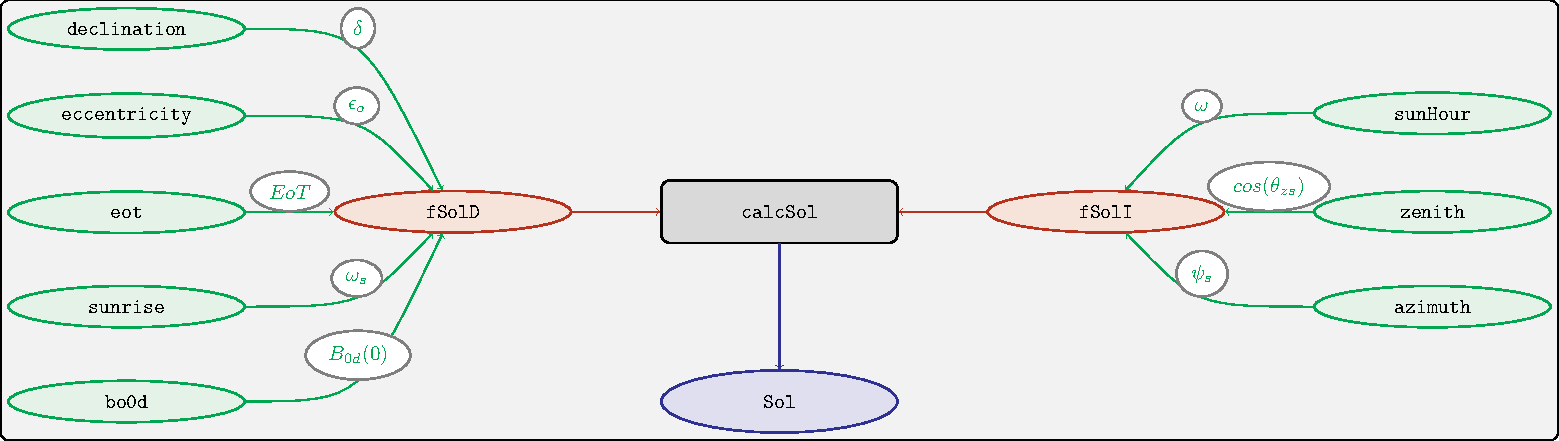
\includegraphics[width=\textwidth]{../figuras/calcsol.pdf}
\end{center}
\end{frame}
\begin{frame}[label={sec:orgb2de32e},fragile]{\texttt{Meteo}}
 \begin{center}
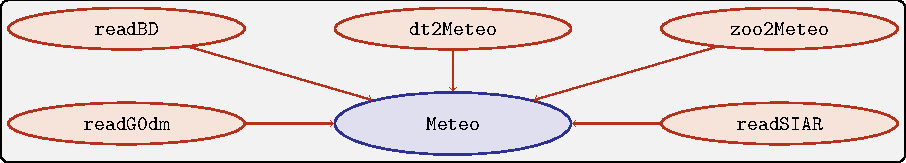
\includegraphics[width=\textwidth]{../figuras/meteo.pdf}
\end{center}
\end{frame}
\begin{frame}[label={sec:orge41e3a1},fragile]{\texttt{calcG0}}
 \begin{center}
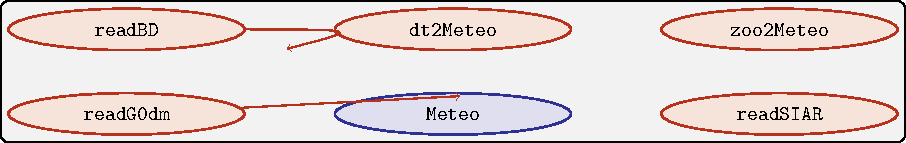
\includegraphics[width=\textwidth]{../figuras/calcg0.pdf}
\end{center}
\end{frame}
\begin{frame}[label={sec:orgc057140},fragile]{\texttt{calcGef}}
 \begin{center}
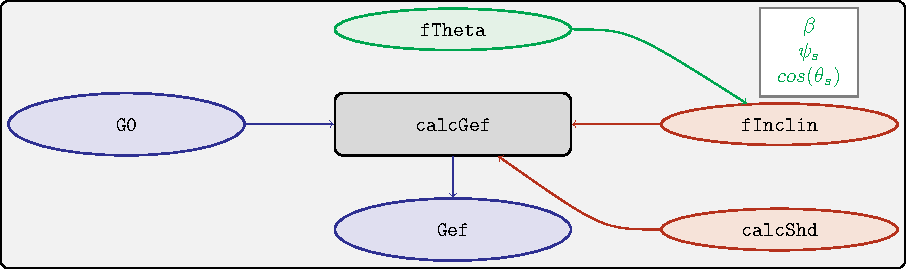
\includegraphics[width=\textwidth]{../figuras/calcgef.pdf}
\end{center}
\end{frame}
\begin{frame}[label={sec:org5358bdd},fragile]{\texttt{prodGCPV}}
 \begin{center}
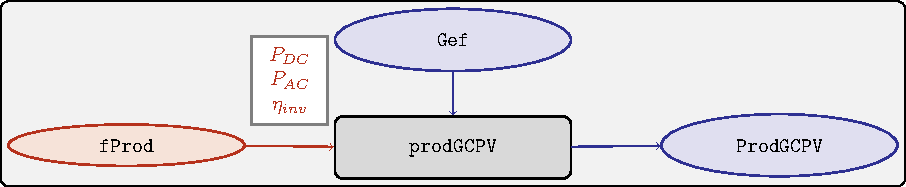
\includegraphics[width=\textwidth]{../figuras/prodgcpv.pdf}
\end{center}
\end{frame}
\begin{frame}[label={sec:orgfa71dca},fragile]{\texttt{prodPVPS}}
 \begin{center}
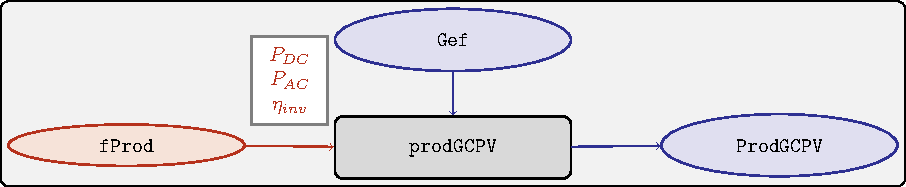
\includegraphics[width=\textwidth]{../figuras/prodpvps.pdf}
\end{center}
\end{frame}
\section{Ejemplo práctico de aplicación}
\label{sec:orgef37413}

\section{Conclusiones}
\label{sec:org36fbc48}
\subsection{Aportaciones}
\label{sec:orgfda848b}
\begin{frame}[label={sec:org999d179}]{Blame}
\begin{center}
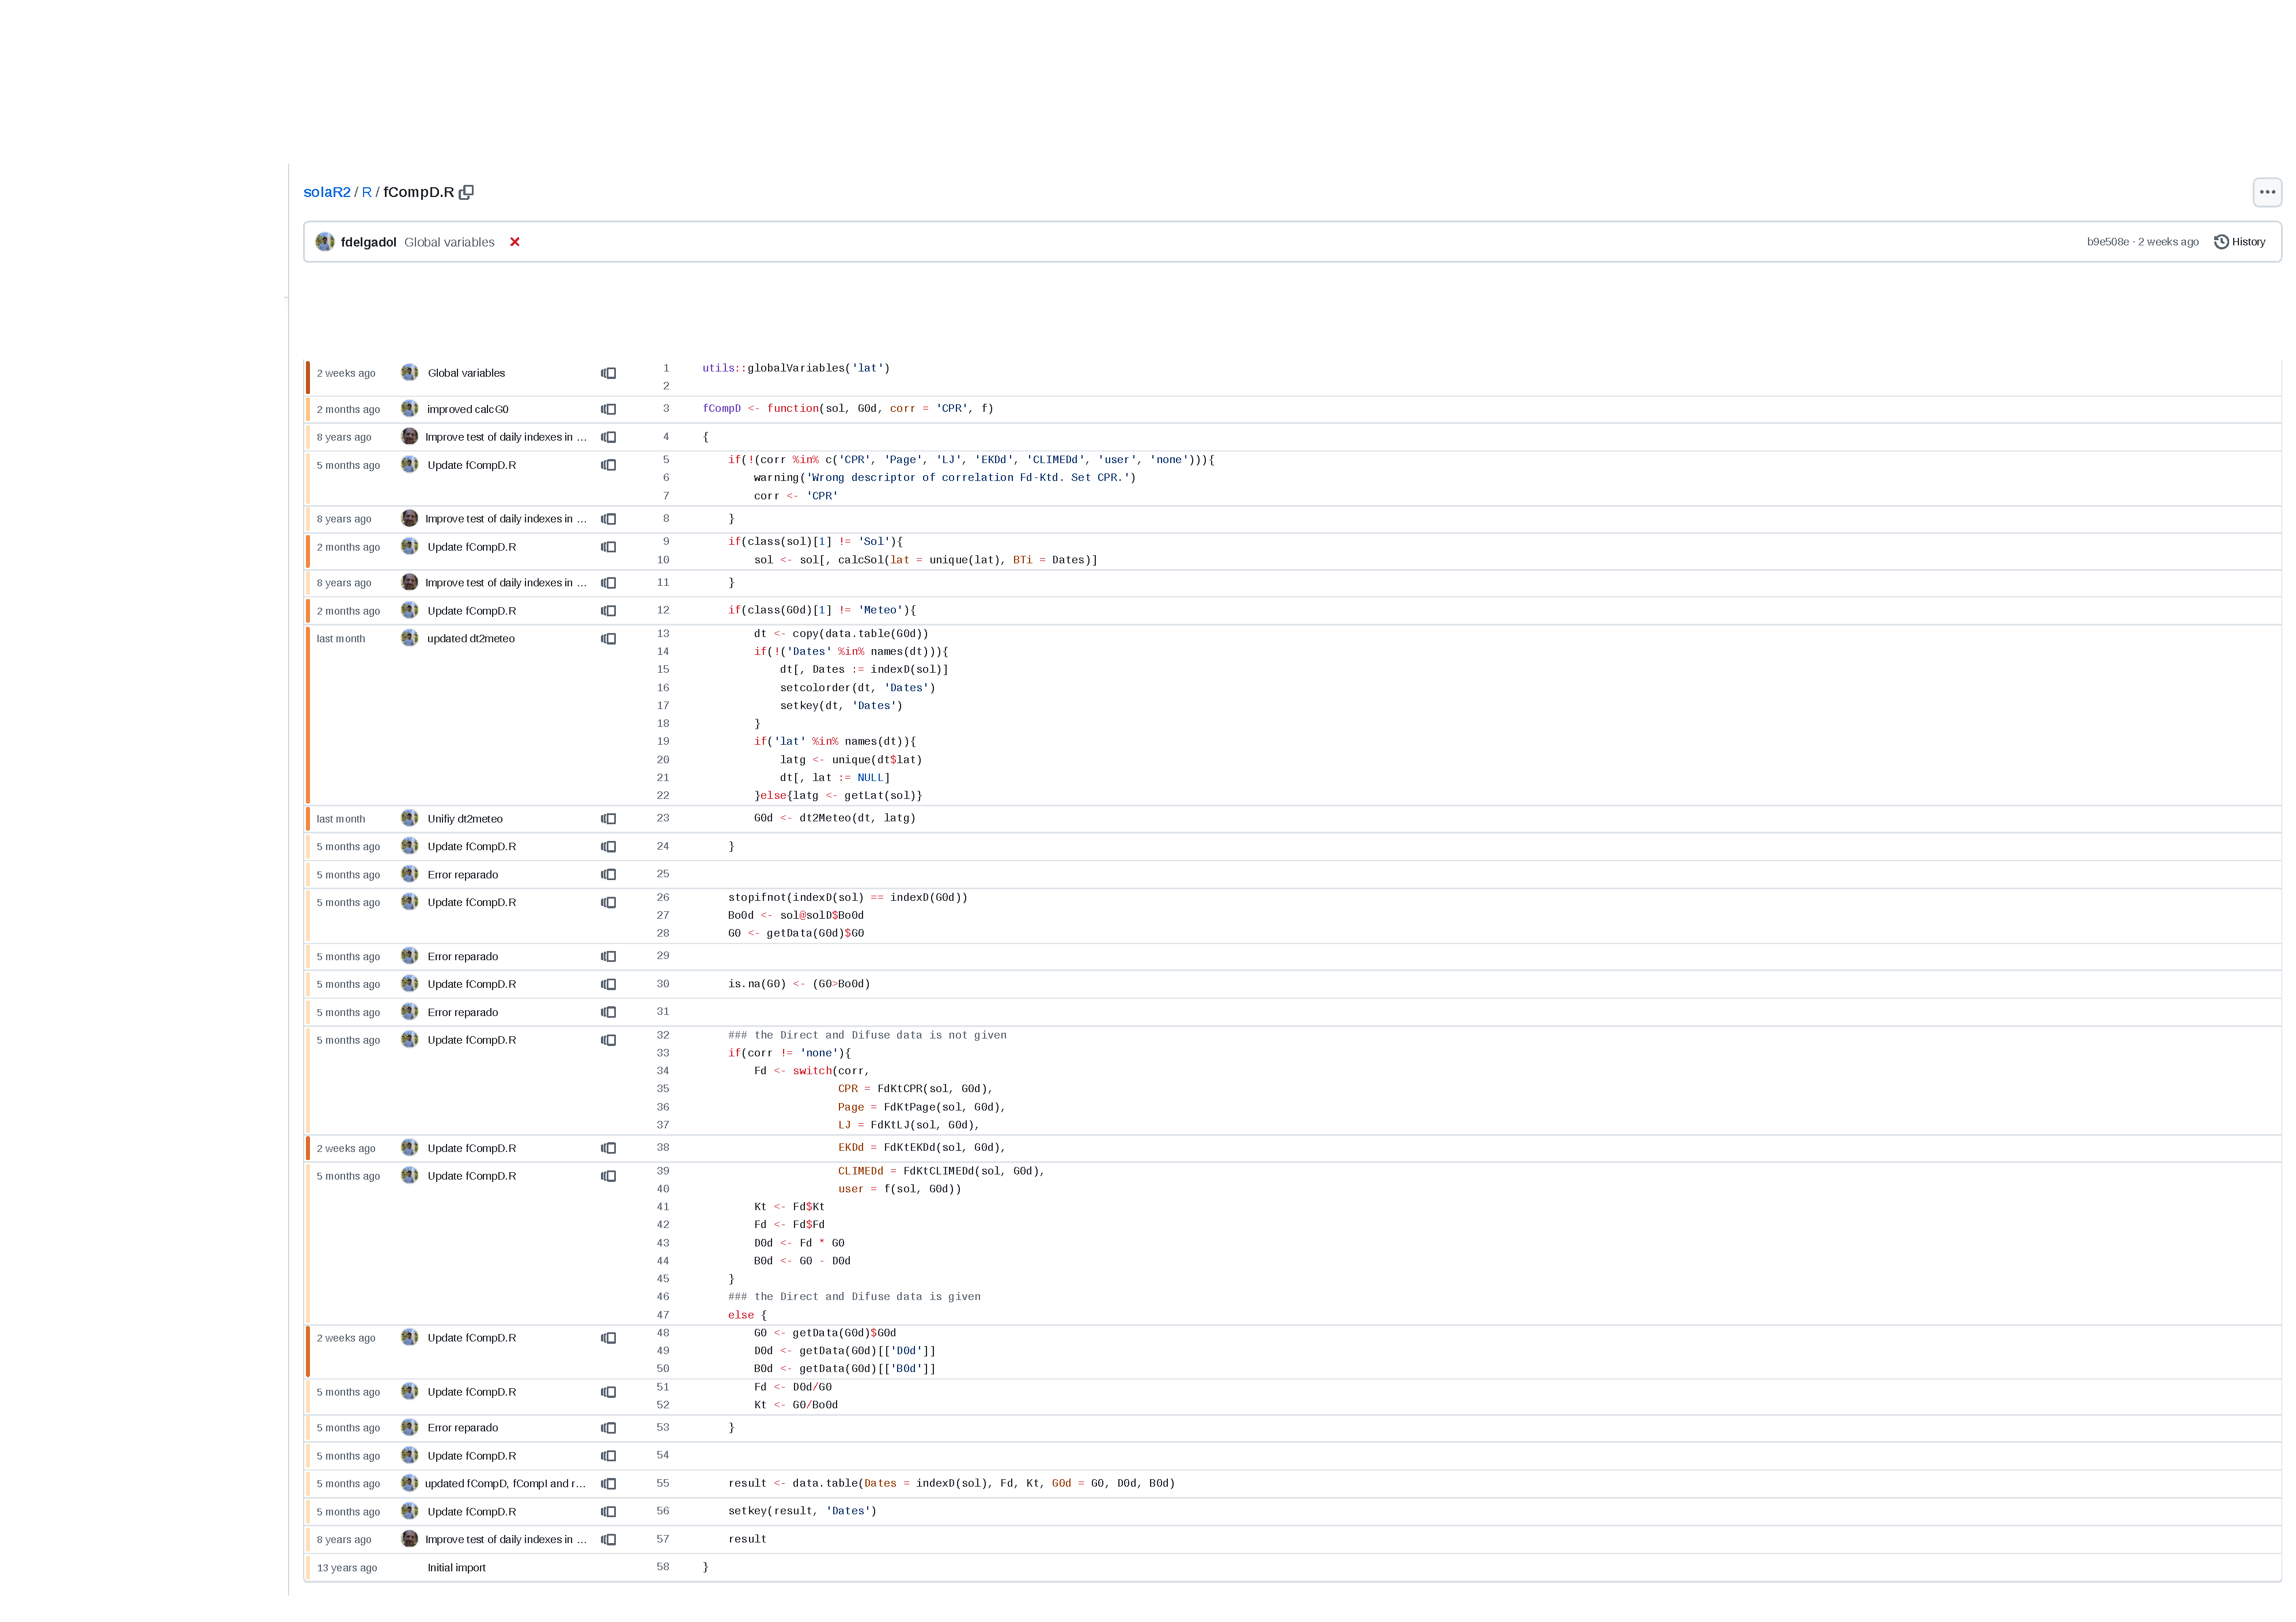
\includegraphics[height=0.9\textheight]{../figuras/blame-fCompD.pdf}
\end{center}
\end{frame}
\begin{frame}[label={sec:org0350899}]{Blame}
\begin{center}
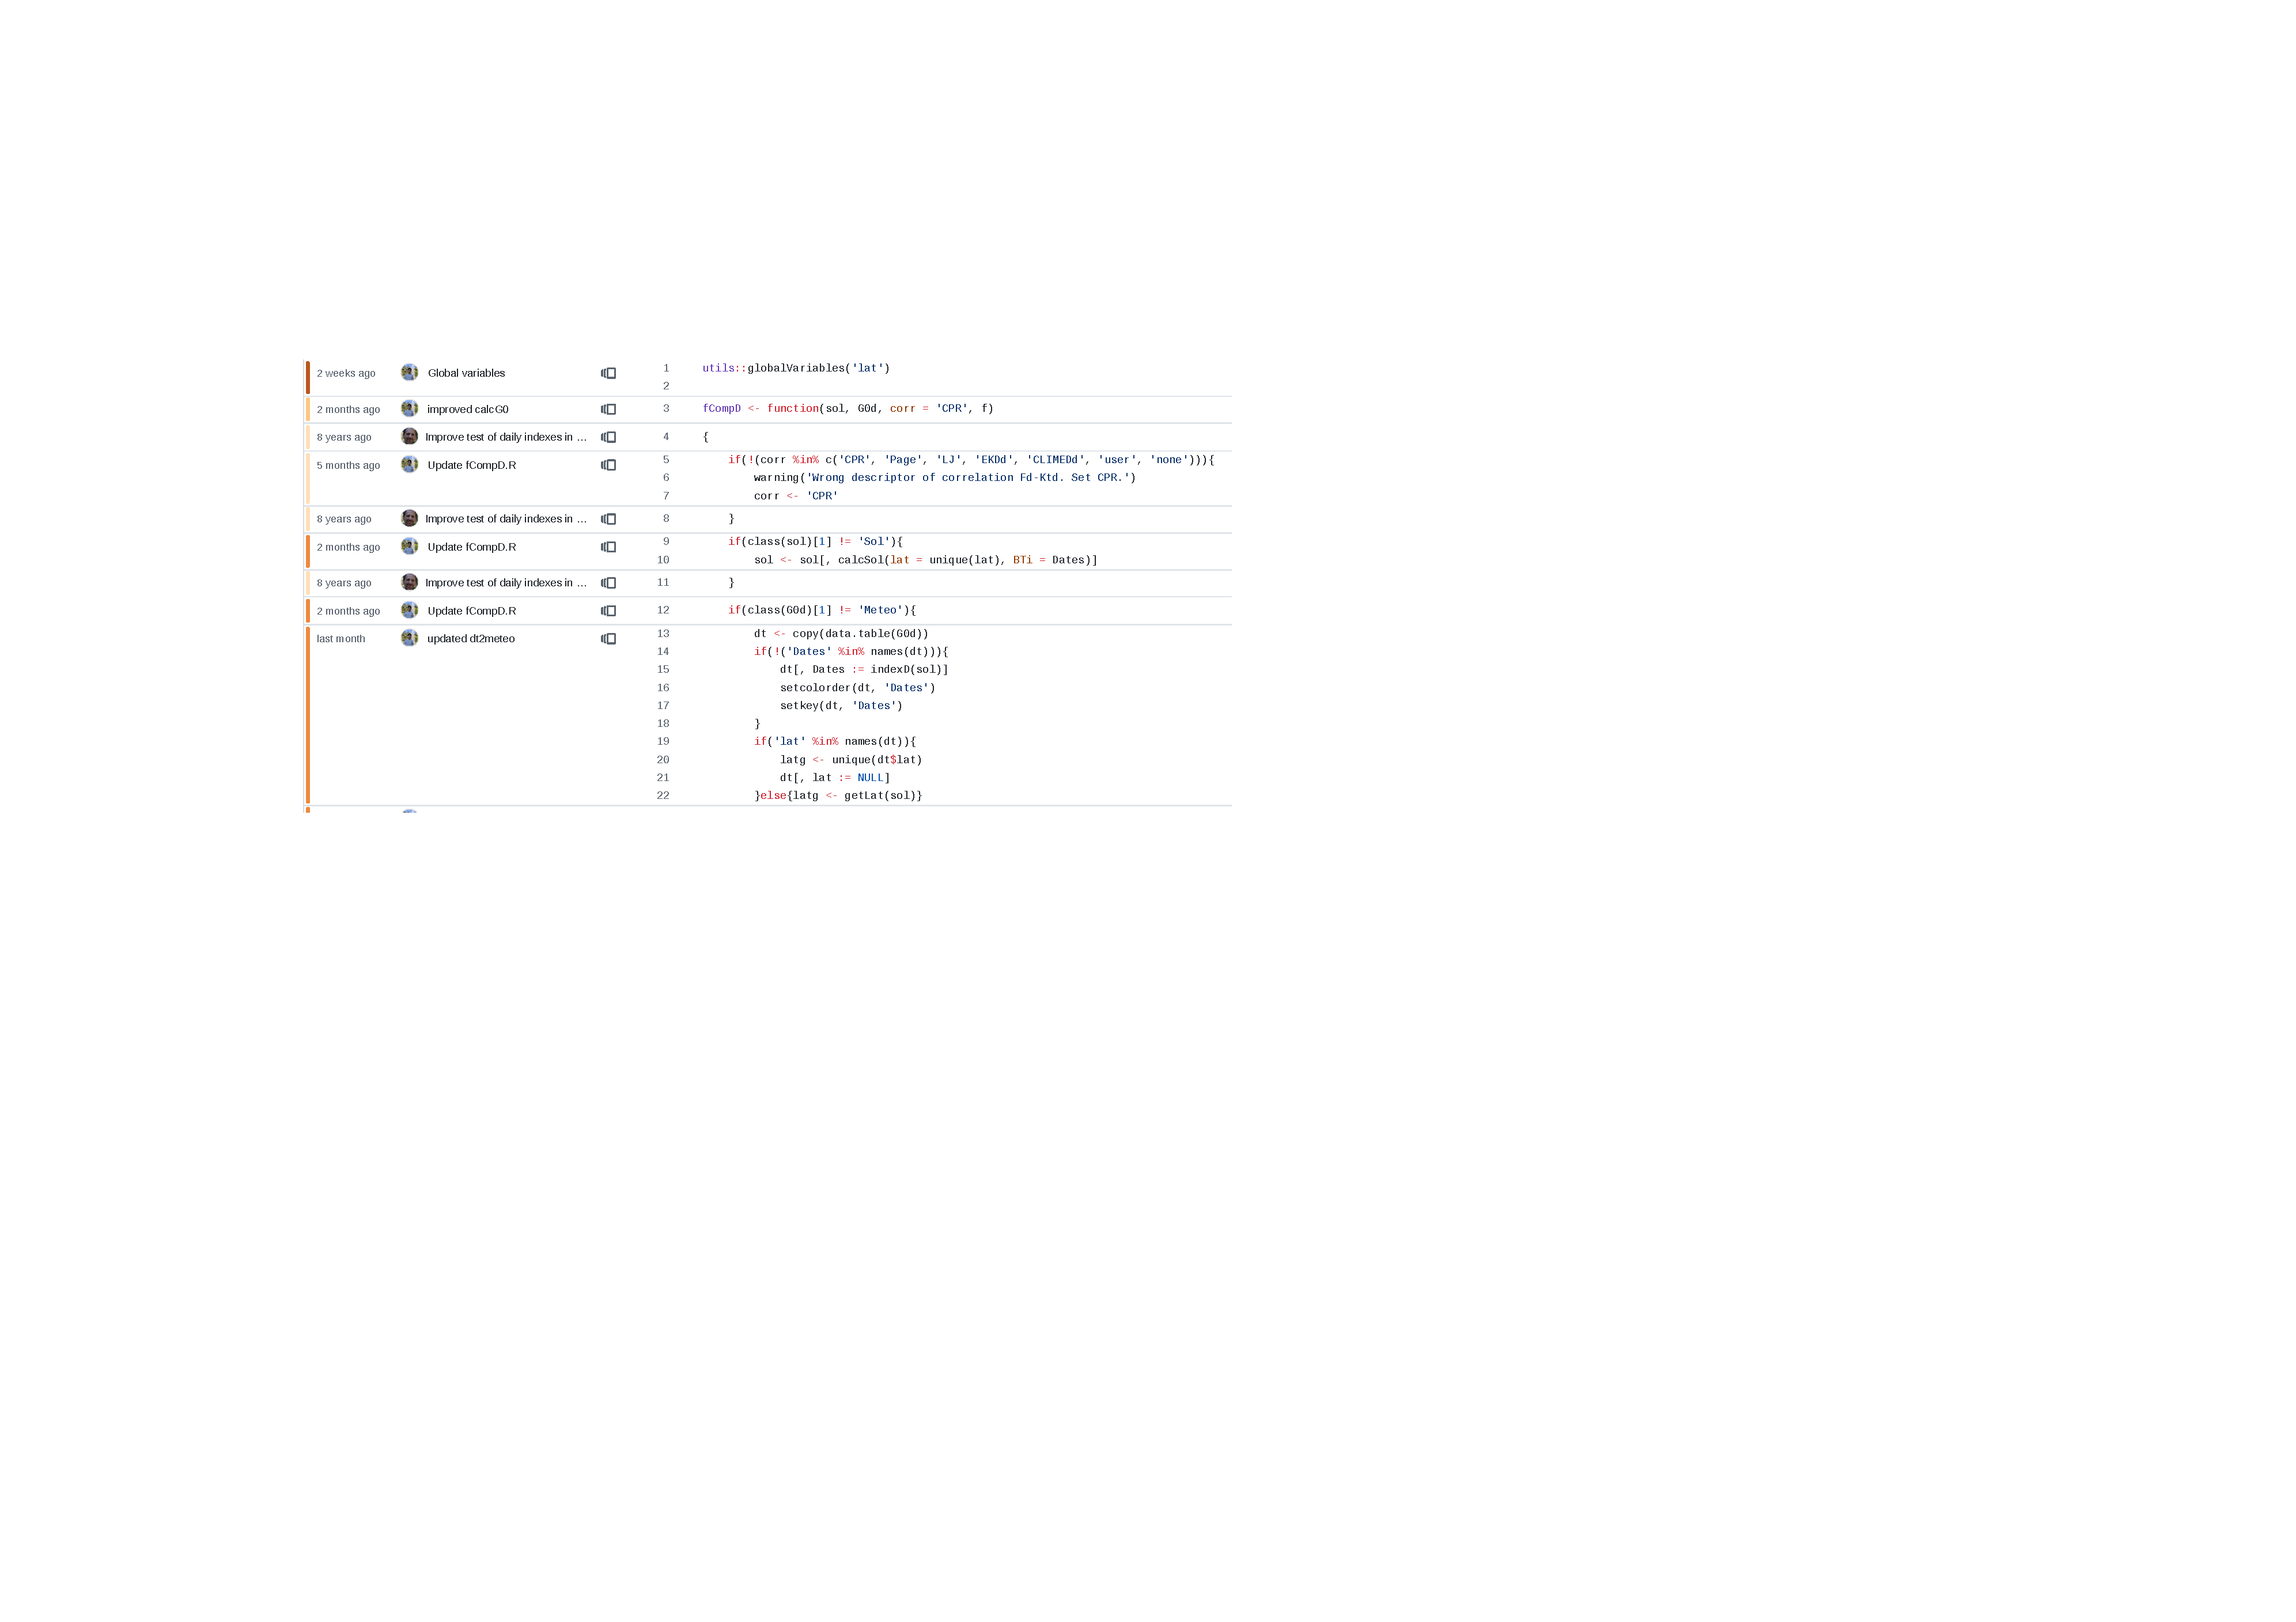
\includegraphics[width=\textwidth]{../figuras/blame-fCompD_cropped.pdf}
\end{center}
\end{frame}
\begin{frame}[label={sec:org987a1e1}]{Insights}
\begin{center}
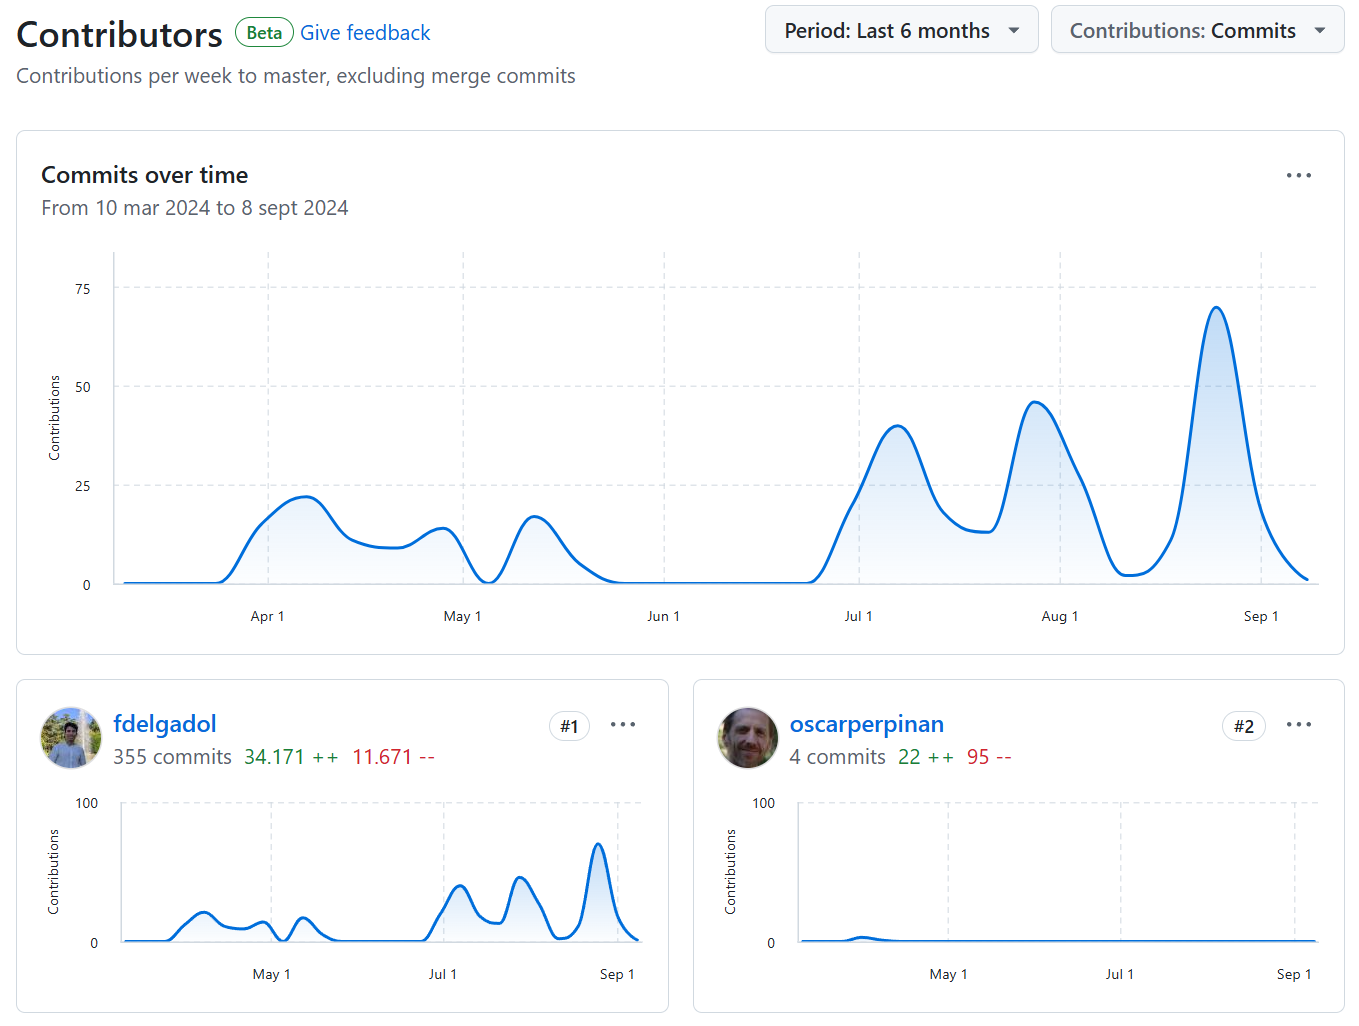
\includegraphics[height=0.9\textheight]{../figuras/contributors.png}
\end{center}
\end{frame}
\subsection{Desarrollo a futuro}
\label{sec:org7f08db7}
\begin{frame}[label={sec:org91c5e0e},fragile]{Desarrollo a futuro}
 \begin{block}{Interfaz de usuario}
\end{block}
\begin{block}{Mejora de funciones}
\end{block}
\begin{block}{Toma de datos}
\end{block}
\begin{block}{Uso de paquete especializados en datos espaciales}
\begin{itemize}
\item \texttt{terra}
\end{itemize}
\end{block}
\end{frame}
\end{document}
